\chapter{Pickup and Deployment Mechanism}
The aim of the project leading up to this master thesis was to explore different design solutions that could be used to facilitate drop and recovery operations of sensor nodes using AUVs. The project report \citep{prosjekt} contains a discussion of different solutions, before concluding upon one solution that was implemented. The implemented solution has been further developed in this master thesis, but most of the concepts remain. Readers are advised to consult the project report for discussions concerning the drop and recovery mechanism, while the resulting, though improved mechanism, is presented in this chapter.
\section{Overall Description}
To get sufficient accuracy in the pickup phase it was decided that a solution where a gripper can be lowered down towards the sensor node was the beast approach. The different parts in this setup was 3D-modeled and 3D-printed. A box was designed to contain the PandaBoard and to mount the gripper mechanism to. A system with gears was designed to be able to lower the gripper in an accurate and reliable fashion. The operation of the mechanism is displayed in Figure \ref{finished}. A camera was mounted to the gripper-platform to be able to track the sensor node and confirm whether the node is picked up or not.
\begin{figure}[H]
\centering
\subfigure[Gripper raised]{
\includegraphics[width=7.95cm]{fig/finished/up.jpg}
\label{up}
}
\centering
\subfigure[Gripper lowered]{
\includegraphics[width=7.95cm]{fig/finished/down.jpg}
\label{down}
}
\caption{Drop and recovery mechanism mounted to the hexacopter}
\label{finished}
\end{figure}
\section{Hardware}
\subsection{IR-LED Position Sensor}
The essence of the IR-LED position sensor is the IR-LED and the photodiode. These need some support circuitry to function. The circuit with the LED is fairly simple. It contains only of the IR-led and a resistor. The resistor is there to limit the current.\\\newline
The circuit for the photodiode is a bit more complicated. The photodiode chosen is a PIN type diode from Everlight. It is connected reversed biased, and does not conduct ordinarily, but starts to conduct when exposed to IR. The more IR the more it conducts. This last fact means that the signal will wary between 0 and 5 V depending on how much IR it ``sees". In this application the LED and the photodiode are mounted in a way that the photodiode only ``sees" the IR when the gripper platform is in position. Hence it is no need for an analog reading, the signal could be connected directly to a digital I/O port to give ether a in position or an out of position value. An opamp used as an voltage follower is included in the design, this isolates the output from the signal source. The operational amplifier used is an MC3405P from Motorola. A resistor is used to limit current.\\\newline
A decoupling capacitor was added. Decoupling capacitors are used to give noise a path to ground and keep the power in the circuit smooth \citep{embedded}. The schematics of the circuit design can be seen in Figure \ref{ledSchematic}. 
\begin{figure}[H]
\centering
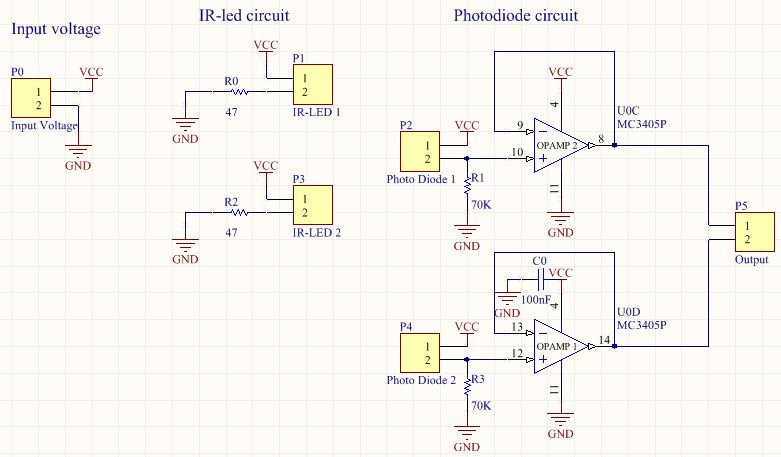
\includegraphics[width = 15cm]{fig/krets/ledSchematic.jpg}
\caption{Schematics for the IR-LED Position Sensor}
\label{ledSchematic}
\end{figure}
\subsection{H-Bridge}
To be able to control direction and speed of the DC-motor lowering and raising the gripper, a H-bridge is needed. The H-bridge chosen for this is the DRV8801 h-bridge motor driver from Texas Instruments mounted to a break out board. The simplicity of this design makes it small in size and very low weight. Nominal output current is rated to 1 A, while it can handle peaks up to 2.8 A for a few seconds. It operates with motor supply voltages between 8 and 36 V and logic supply voltages between 3.3 and 6.5 volts \citep{h-bridge}. This makes it very versatile. The main drawback with the simplicity of this chip and break out board is that it could quite easily get over heated if driven with high current over time. This should not be a problem in this application because the nominal current of the chosen motor is given to be 50 mA and the time used to lower or raise the gripper is limited.
\subsection{Level Translator}
\label{level}
Communication will go both to and from the PandaBoard. The level translator will need at least eight channels, three for controlling the H-bridge, one for servo control, two for UART and two for the IR-LED position sensor signals. For this reason the  ADG3300BRUZ eight channel bidirectional level translator from Analog Devices was chosen. It is a convenient and easy to use level translator, just connect the desired low voltage and low voltage signals at one side and the desired hight voltage and high voltage signals at the other side. Two decoupling capacitors are also connected. The schematics of the circuit design can be seen in Figure \ref{levelTranslatorSchematic}.
\begin{figure}[H]
\centering
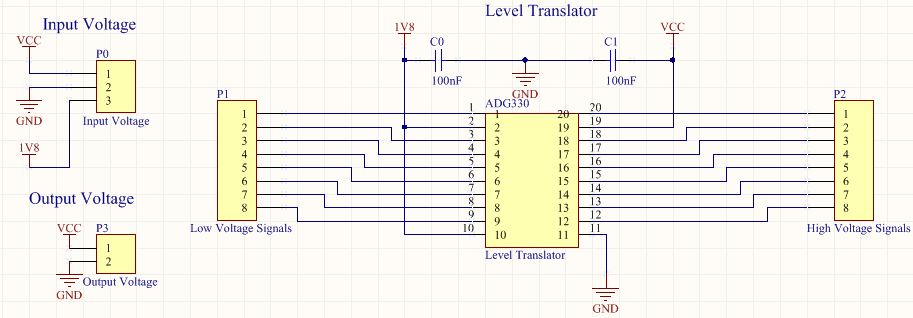
\includegraphics[width = 15cm]{fig/krets/levelTranslator.jpg}
\caption{Schematics for the Level Translator}
\label{levelTranslatorSchematic}
\end{figure}
\subsection{PWM-Controller}
The servo mounted to the gripper is controlled by using a PWM\footnote{Pulse Width Modulated}-signal. Where the time where the signal is high is transferable to the servos position reference. Typically is the time period for PWM signals controlling RC equipment 20 ms. With a high pulse of 1 ms meaning 0 degrees and 2 ms meaning 180 degrees. This means that to be able to control the servo in a stable and accurate way, the PWM-signal needs to be accurate. To get such an accurate signal using the PandaBoard can be challenging. It is possible to 
generate PWM with the PandaBoard using GPIO-pins and a real time operating system. But the operating system running on the PandaBoard in this project is a stripped down version of a Linux kernel without real time possibilities. In addition will the gripper be controlled through which further increases difficulties with timing.\\
\newline
To cope with this problems a PWM-controller was designed. The basis for the PWM-controller is an ATtiny85 8-bit microcontroller. This microcontroller is chosen for its simplicity. The microcontroller is programmed using ISP. To be able to program the microcontroller in circuit pins are added to all the pins, even though not all will be used in the application. This will also increase the possibilities for further developing if needed. A decoupling capacitor was also added to ensure noise free input voltage for the microcontroller.\\
\newline
Two bits will be used to control the PWM-controller with the PandaBoard. One bit turns on and off the signal, while the other bit gives the desired position of the gripper (either open or closed). The schematics of this circuit is shown in Figure \ref{pwm}, while the code running on the ATtiny85 is included in the digital appendix.
\begin{figure}[H]
\centering
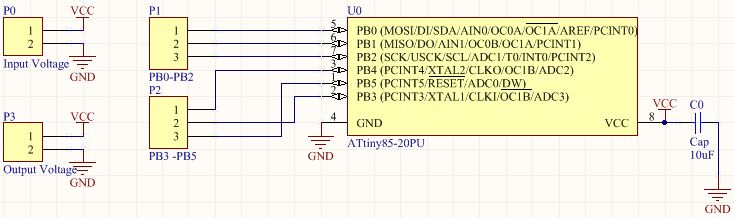
\includegraphics[width = 16cm]{fig/krets/pwm.JPG}
\caption{Schematics for the PWM-Controller}
\label{pwm}
\end{figure}\noindent
\section{Communication Between the Modules}
An overview of the different modules and the communication between them is shown in Figure \ref{com}.\\
\newline
The PandaBoard communicates with the camera through a dedicated port that uses the MIPI CSI-2 standard. The rest of the communication to and from the PandaBoard goes via the level translator described in the previous section. The servo for the gripper is controlled with a PWM-signal while the H-bridge is controlled using three digital outputs. The communication between the PandaBoard and the APM uses UART and the MAVLink protocol. Relevant information here will be attitude and position data, and set points for the controller in the APM.
\begin{figure}[H]
\centering
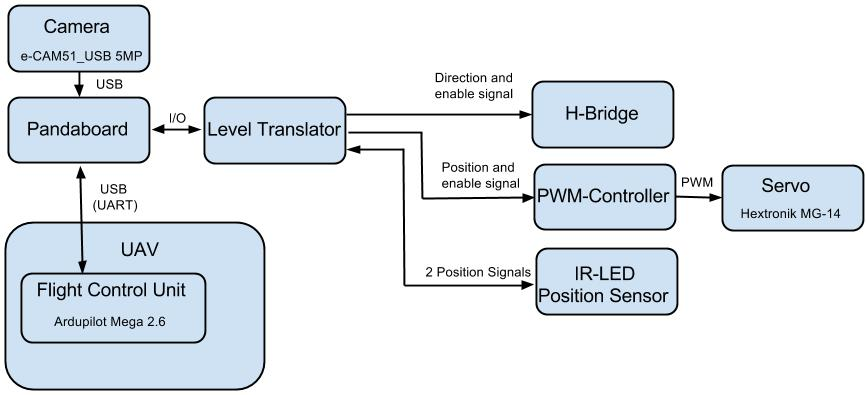
\includegraphics[width = 12cm]{fig/krets/com.jpg}
\label{com}
\caption{Communication between the modules}
\end{figure}
\section{Power Supply}
The UAV contains a battery and a voltage regulator that regulates the voltage down to 5 V. It is possible to use this voltage source for the parts developed in this project. But using the regulated voltage source could easily result in to much current drawn, which will result in restarts of the APM and the Pandaboard. This could be disastrous for the UAV. To avoid this problem one could use a dedicated voltage regulator for the parts developed in this project, but that will decrease the range of the UAV and increase the chance of losing the UAV in case of problems with the parts developed in this project. Hence the safest and best solution is to add a separate battery and voltage regulator, this will increase weight which  will reduce range of the UAV, but this is considered to be a reasonable trade-off. To be able to decide which battery and voltage regulator to use, power demands are investigated and summarized in Table \ref{powerNeeds}.
\begin{table}[H]
\caption{Power demands}
\begin{center}
    \begin{tabular}{| l | l | l | l | l |}
    \hline
    \bf{Unit} & \bf{Voltage [V]} & \parbox{1.5cm}{\bf{Current} \bf{Peak [mA]}} & \parbox{1.5cm}{\bf{Current}\\ \bf{Normal [mA]}} & \bf{Source of info} \\ \hline
    Pandaboard & 5 & 1200 & 700\footnote{Based on tests of an earlier version of PandaBoard with CPU running at a 100 \% \cite{pandaboard_test}}& \parbox{4cm}{Pandaboard FAQ\\\citep{pandaboard}}\\ \hline
    Servo & 5 & 1500 & 800 & Measured\\ \hline
    DC motor & 12 & 50 & 50 &\parbox{4cm}{Data sheet \\\citep{motor}}\\ \hline
    Level Translator & 5 and 1.8 & 0.17E-3 & 5E-3 & \parbox{4cm}{Data sheet\\\citep{adg3300}}\\ \hline
    IR-LED Position Sensor & 5 & 150 & 450 & Measured\\ \hline
    Camera & 5 & 150 & 150 & \parbox{4.2cm}{Manufacturer web page\\\citep{camera_power}}\\\hline
    \bf{SUM} & - & \bf{3050} & \bf{2150} &\\\hline
    \end{tabular}
    \label{powerNeeds}
\end{center}
\end{table}\noindent
Selecting battery is a trade-off between capacity and weight. The battery should be able to power both the motor and the ICs\footnote{Integrated Circuits}. Hence a three cell Lithium-Polymer battery is chosen. These kind of batteries deliver 11.1 V, are able to deliver a lot of power fast and able to hold a lot of power in relation to its weight. The specific battery chosen is a 1000 mAh 20-30 C (means that it is able of delivering an instantaneous current of 20-30 times the capacity) battery from Haiyin. The battery is able to support the peak currents, but it might not be able to operate for very long if the servo and motor is used a lot in the mission. The battery will be replaced by a heavier one with greater capacity if necessary.\\
\newline
To reduce the chance for unstable voltages and current delivered to the PandaBoard, two voltage regulators are used, one for the PandaBoard and one for the rest of the equipment. Especially the servo can be a cause for ripple in the delivered voltage and current. This choices result in the power circuit displayed in Figure \ref{powerCircuit}.
\begin{figure}[H]
\centering
\includegraphics[width = 16cm]{fig/krets/power.jpg}
\caption{Power circuit}
\label{powerCircuit}
\end{figure}
\section{Camera Application}
The main application of the camera is to track the sensor node. The camera will also be used in the pickup to verify whether the gripper got hold of the sensor node or not (one could have used estimation of inertia for this task like \citep{Mellinger2011}, but the position of the camera makes it very convenient to use for this task). To be able to track the sensor node the camera will need to recognize the sensor node. This can be done in multiple ways as described briefly in Section \ref{opencv}. The SURF method can be efficient under the right circumstances, but some simple tests revealed some weaknesses. It turned out that only a few points on a picture of the pickup mount was marked as corners that it could use to search for. Of course the pickup mount could be made in a way that it would have more detail, but because it is quite small and it should be possible to detect at a distance this method was discarded. A classifier could be developed, but it will have weaknesses when it comes to rotation, and it would need a lot of example pictures to make it robust. Of this reasons the classifier solution was discarded as well. The much simpler solution of color detection was implemented.
\subsection{Tracking the Sensor Node}
\label{node}
To be able to use color detection the sensor node need to have some colors that sticks out. The mount for the sensor node (Figure \ref{sensorNode}) should have two different colors to make it possible to use color detection to get the orientation of the mount. The ocean is blue, which means that the sensor node should have colors that are as far away from blue on the HSV-wheel (Figure \ref{hsvWheel}). Yellow is an obvious choice because it is directly opposite of blue and it has a narrow band, which is good for noise cancellation. The colors next to yellow is red and green. Red contains both the lowest an highest hue values, which will make calculations more complex, hence green is chosen for the other color.\\
\newline
The picture from the camera is converted to the HSV-color space and copied to create two pictures. One of the pictures is thresholded with the HSV-values for yellow, while the other is thresholded with the values for green. This creates two binary pictures where the yellow and green fields are marked respectively. Then the "center of mass" of the two pictures are calculated. This centres of masses are used as centres of the two parts of the pickup mount and used to calculate the orientation of the mount and the center of the mount. This procedure is demonstrated in Figure \ref{color}. These points are in the picture frame. For the measurements to make sense one need a mapping from this pixel position to the position of the mount in NED.\\
\begin{figure}[H]
\centering
\subfigure[Original image]{
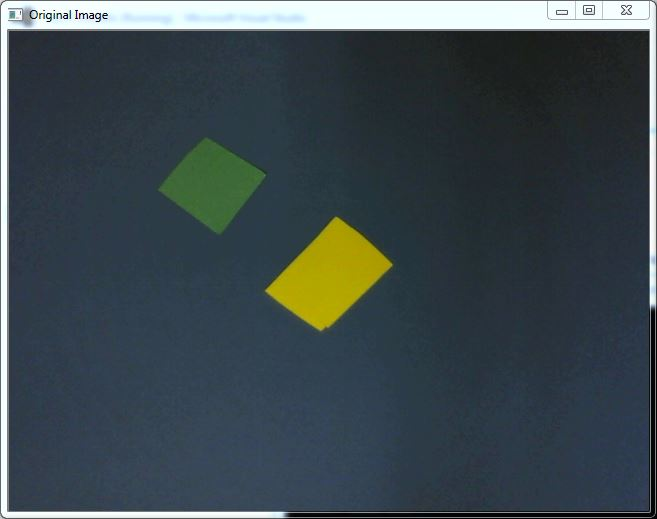
\includegraphics[width=7cm]{fig/colorRecognition/original.jpg}
}
\centering
\subfigure[HSV image]{
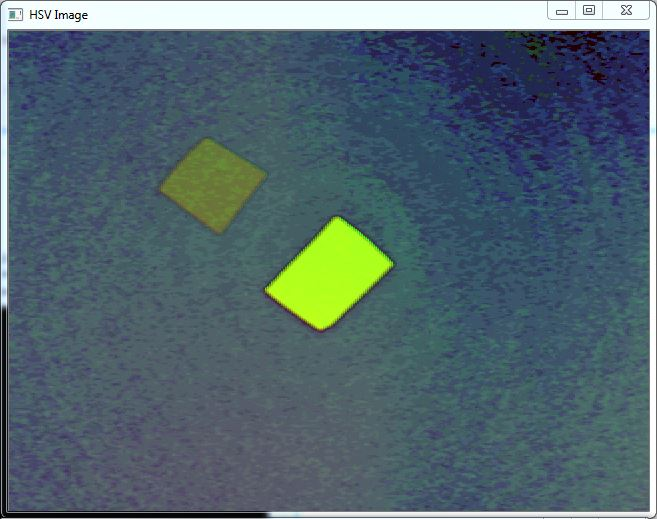
\includegraphics[width=7cm]{fig/colorRecognition/hsv.jpg}
}
\centering
\subfigure[Green thresholded]{
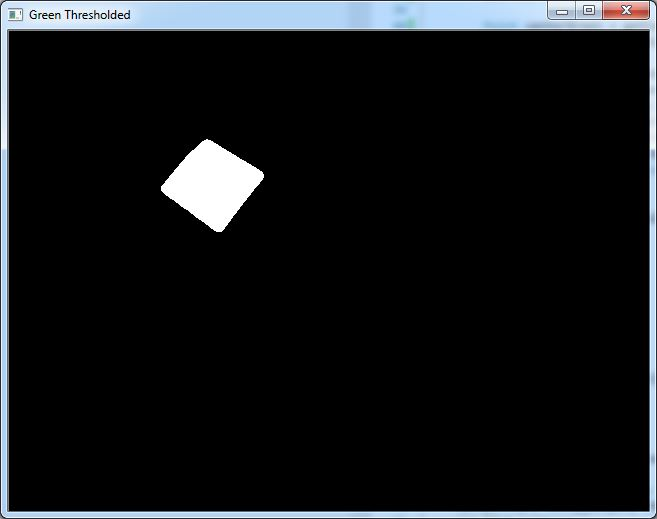
\includegraphics[width=7cm]{fig/colorRecognition/green.jpg}
}
\centering
\subfigure[Yellow thresholded]{
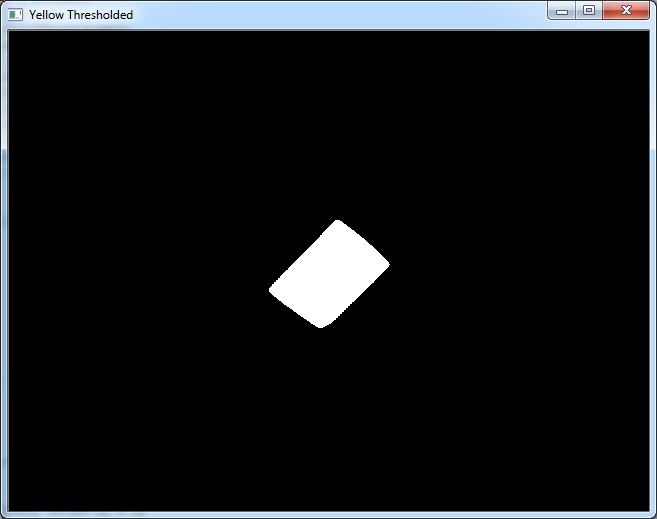
\includegraphics[width=7cm]{fig/colorRecognition/yellow.jpg}
}
\centering
\subfigure[Result]{
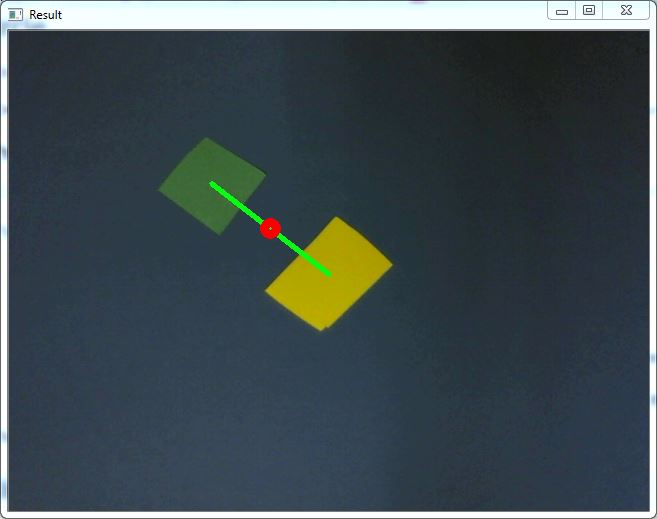
\includegraphics[width=7cm]{fig/colorRecognition/result.jpg}
}
\caption{Use of color recognition to track the mount of the sensor node}
\label{color}
\end{figure}\noindent
For control purposes a position of the sensor node in NED is good because this will be the same value as the error in position if the controller is trying to get to the exact position of the sensor node. For estimator and robustness the sensor nodes position should be referenced in ECEF. If the position of the sensor node is referenced in ECEF, it will be simpler to filter out weird measurements, estimation of the movements of the sensor node with current and waves becomes possible and the controller will have something to navigate towards even if the camera looses sight of the sensor node for a moment.\\\newline
To get the position of the sensor node in NED, first a transformation from BODY to NED is conducted by the use of the rotation matrix from BODY to NED in equation (\ref{R_ned}). DH convention is used to create consequential reference frames from BODY leading up to a reference frame in the sensor node. This is done to exploit the fact that the transformation matrix from BODY to the sensor node reference frame will contain the position of the sensor node reference frame expressed in BODY as seen in equation (\ref{T}).\\\newline
The first new frame is defined in the center of the camera lens. The homogeneous transformation $A_1$ from BODY to the camera frame is carried out as a movement $d_1$ along the BODY z-axis which gives the relation below. This coordinate frame and subsequent frames are visualized in Figure \ref{camera}. The parameters related to the transformations are also marked in the same figure.
\begin{eqnarray}
\boldsymbol{A}_1 = \begin{bmatrix}
1 & 0 & 0 & 0\\
0 & 1 & 0 & 0\\
0 & 0 & 1 & d_1\\
0 & 0 & 0 & 1
\end{bmatrix}
\end{eqnarray}
The next coordinate system is defined with the z-axis pointing towards the sensor node and the pixel position of the sensor node in the picture frame. This is done by rotating around the z-axis of $\alpha$ degrees and then rotating around the x-axis of $\beta$ degrees.\\\newline
To find $\alpha$ and $\beta$ some calculations needs to be done. The origin of the picture plane is in the topmost left corner. To get the angles to rotate, the origin is moved to the center of the picture frame by defining $\delta x = x_o - x_c$ and $\delta y = y_o - y_c$. The center of the picture frame is the point $(x_c, y_c)$ while the pixel position of the sensor node is the point $(x_o, y_o)$. The picture frame is defined to be at a distance of one meter away from the camera lens and the length between each pixel at this distance ($L$) is measured using an object of known length. The angles $\alpha$ and $\beta$ are then calculated.
\begin{eqnarray}
\alpha &=& atan2(\delta y, \delta x)\\
d &=& L\sqrt{\delta x^2 + \delta y^2}\\
\beta &=& \tan ^{-1}(d)\\
\end{eqnarray}
The resulting homogeneous transformation matrix is
\begin{eqnarray}
\boldsymbol{A}_2 = \begin{bmatrix}
c_\alpha & -s_\alpha & 0 & 0\\
s_\alpha & c_\alpha  & 0 & 0\\
0		 & 0		 & 1 & 0\\
0 		 & 0		 & 0 & 1
\end{bmatrix}
\begin{bmatrix}
1 & 0 		& 0 	   & 0\\
0 & c_\beta & -s_\beta & 0\\
0 & s_\beta & c_\beta  & 0\\
0 & 0		& 0		   & 1
\end{bmatrix}
= \begin{bmatrix}
c_\alpha	& -s_\alpha c_\beta		& s_\alpha s_\beta 		& 0\\
s_\alpha	& c_\alpha c_\beta	 	& -c_\alpha s_\beta 	& 0\\
0			& s_\beta			 	& c_\beta 				& 0\\
0			& 0						& 0						& 1
\end{bmatrix}
\end{eqnarray}
The last reference frame is defined in the sensor node. To get there a movement of $d_2$ along the z-axis is necessary. To calculate this distance, the angle ($\gamma$) between the z-axis in NED and the z-axis in the picture frame reference system needs to be calculated. The transformation matrix from NED to picture frame is calculated to be able to read out the direction of the z-axis in the picture frame reference system.
\begin{eqnarray}
\boldsymbol{T}_{pf}^{n} = \boldsymbol{R}_b^n(\boldsymbol{\Theta} _{nb})\boldsymbol{A}_1\boldsymbol{A}_2
\end{eqnarray}
Out of this transformation matrix one can read out the direction of the z-axis of the picture frame reference system $\boldsymbol{z} _{pf}^n$ while the direction of the z-axis of NED is trivial.
\begin{eqnarray}
\boldsymbol{z}_{pf}^n = \begin{bmatrix}
s_\alpha s_\beta c_\psi c_\theta - c_\alpha s_\beta (-s_\psi c_\phi + c_\psi s_\theta s_\phi) + c_\beta (c_\psi c_\phi + s_\psi s_\theta s_\phi)\\
s_\alpha s_\beta s_\psi c_\theta -c_\alpha s_\beta (c_\psi c_\phi + s_\psi s_\theta s_\phi) + c_\beta (-c_\psi s_\phi + s_\psi s_\theta s_\phi)\\
-s_\alpha s_\beta s_\theta - c_\alpha s_\beta c_\theta s_\phi + c_\beta c_\theta c_\phi
\end{bmatrix}
	\boldsymbol{z}_n^n = \begin{bmatrix}
	0\\0\\1
	\end{bmatrix}
\end{eqnarray}
The angle $\gamma$ between these two vectors can be calculated using dot product, and the fact that the vectors in the rotation matrices are normalized. This combined with basic trigonometry gives these two relations.
\begin{eqnarray}
\cos \gamma &=& \dfrac{\boldsymbol{z}_{pf}^n\cdot \boldsymbol{z}_n^n}{|\boldsymbol{z}_{pf}^n||\boldsymbol{z}_n^n|} = z_{pf_3}^n\\
\cos\gamma &=& \dfrac{h - d_1c_\theta c_\phi}{d_2}
\end{eqnarray}
These relations combined gives the following expression for $d_2$ and the homogeneous transform.
\begin{eqnarray}
d_2 &=& \dfrac{h - d_1c_\theta c_\phi}{z_{pf_3}^n}\\
\boldsymbol{A}_3 &=& \begin{bmatrix}
1 & 0 & 0 & 0\\
0 & 1 & 0 & 0\\
0 & 0 & 1 & d_2\\
0 & 0 & 0 & 1
\end{bmatrix}\\
\boldsymbol{T}_{obj}^n &=& \boldsymbol{T}_{pf}^{n}\boldsymbol{A}_3
\label{T_last}
\end{eqnarray}
Calculations of equation (\ref{T_last}) will read out the position of the origin of the reference frame in the sensor node (according to equation (\ref{T})). This gives
\begin{eqnarray}
\boldsymbol{p}_{obj}^n = \begin{bmatrix}
d_2z_{pf_1}^n + d_1(s_\psi s_\phi + c_ \psi s_\theta c_\phi)\\
d_2z_{pf_2}^n + d_1(-c_\psi s_\phi + s_\psi s_\theta c_\phi)\\
h
\end{bmatrix}
\end{eqnarray}
For the purpose of tracking this vector is then transformed into the ECEF coordinate frame by the transform in equation (\ref{ecef}).
\begin{figure}[H]
\centering
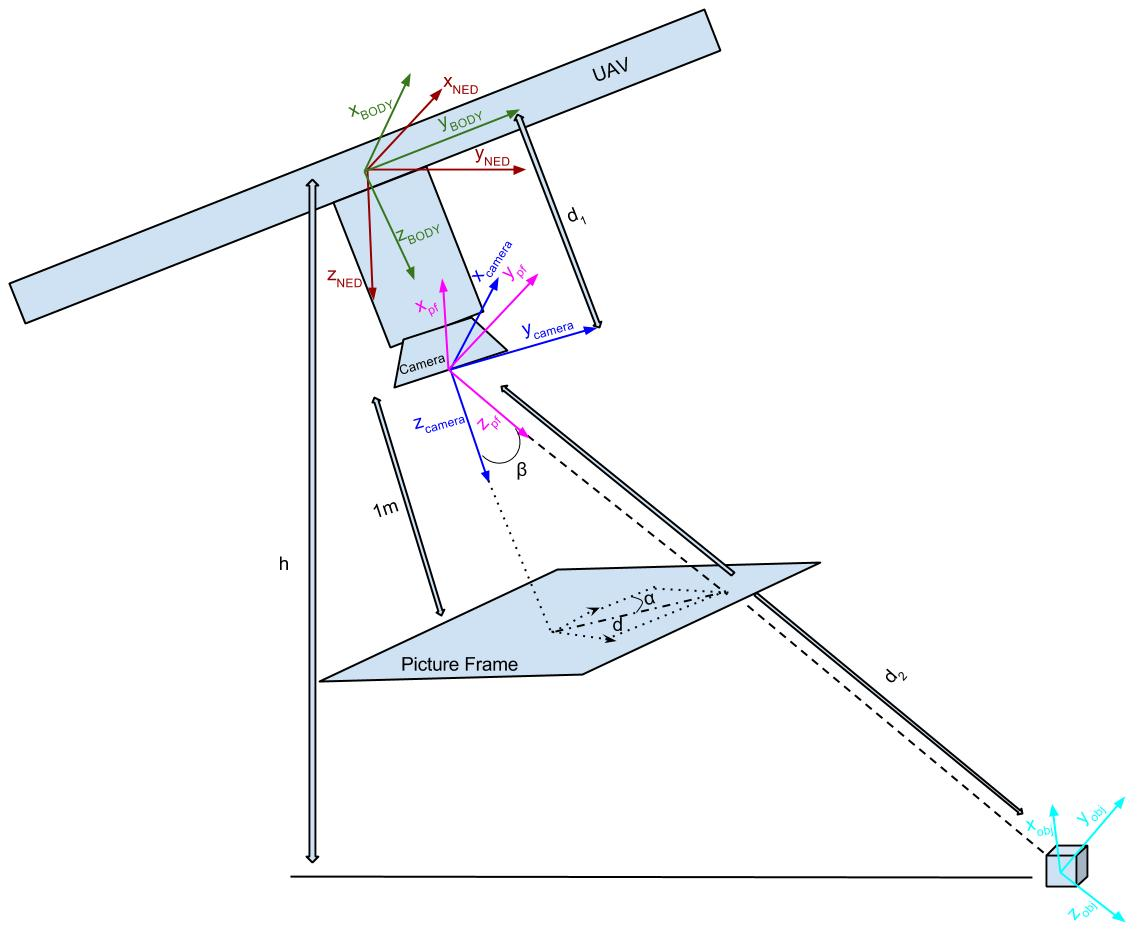
\includegraphics[width = 18cm]{fig/camera.jpg}
\caption{Visualization of the different coordinate systems}
\label{camera}
\end{figure}
